\chapter{\LaTeX 环境搭建}
\section{安装发行版}
\LaTeX
是一个非常庞杂的系统,里面涉及到各种各样的编译器,引擎,宏包,如果自己要手动去安装这些的话是非常麻烦的。发行版把这些内容全部打包,对应不同的操作系统有不同的版本,大大降低了配置的难度。
\begin{table}[htpb]
	\centering
	\begin{tabular}{ lll } \toprule
		系统       & 发行版   \\          \midrule
		Windows    & MikTeX   \\
		Unix/Linux & Tex Live \\
		macOS      & MacTeX   \\\bottomrule
	\end{tabular}
	\caption{\LaTeX 发行版与编辑器}
\end{table}

发行版的安装可以直接搜索对应的官网下载,然后安装即可。如果需要详细的指导,可以搜索``\href{https://mirrors.concertpass.com/tex-archive/info/install-latex-guide-zh-cn/install-latex-guide-zh-cn.pdf}{一份简短的关于 LATEX
	安装的介绍}\footnote{https://mirrors.concertpass.com/tex-archive/info/install-latex-guide-zh-cn/install-latex-guide-zh-cn.pdf}''。这份文档也包含在发行版中,如果你已经安装了发行版,可以在命令行中输入以下内容来找到此文档:
\begin{shellcmd}
	texdoc install-latex-guide-zh-cn
\end{shellcmd}

\section{编辑器}
\LaTeX 文件是纯文本格式,所以理论上讲任何文本编译器都能用来写\LaTeX 代码。实际操作中,快速的写出漂亮优雅的\LaTeX
代码需要编辑器具备语法高亮,自动补全,语法错误提示,格式化代码,自动编译等一系列的功能。所以一个好的编辑器是必不可少的。

下表数据来自\href{https://en.wikipedia.org/wiki/Comparison_of_TeX_editors}{维基百科}\footnote{https://en.wikipedia.org/wiki/Comparison\_of\_TeX\_editors},我删除了一些我认为不重要的项目。如果你不方便安装的话,可以尝试使用overleaf的在线编辑器。

\begin{table}[thpb]
	\centering
	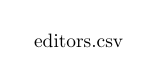
\begin{tikzpicture}
		\node[scale=0.7] {\csvautobooktabular{editors.csv}};
	\end{tikzpicture}

	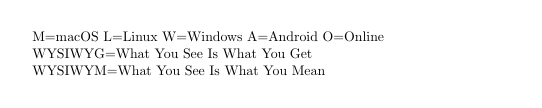
\begin{tikzpicture}
		\node[scale=0.5, text width=\textwidth]{
			M=macOS L=Linux W=Windows A=Android O=Online \\
			WYSIWYG=What You See Is What You Get         \\
			WYSIWYM=What You See Is What You Mean        \\};
	\end{tikzpicture}
	\caption{编辑器功能对照表}
\end{table}

编辑器本身也有一定的学习成本,大家最开始不妨使用发行版自带的,以后可以多试几个,找一个自己使用得顺手的。如果你对编程的编辑器熟悉的话,可以试试用VS
Code + LaTeX Workshop。Vim + vimtex也是一个不错的方案,不过上手难度较大,新手不建议。

\section{PDF文件浏览器}
文件浏览器主要考虑两点,一、兼容性,能不能正确显示文件里面的内容;二、阅读时控制是否方便。Adobe Acrobat Reader
是一个广泛使用的 PDF 阅读器,它提供了丰富的功能和良好的兼容性。然而,还有许多其他优秀的PDF阅读器,如 Foxit
Reader、Sumatra PDF、PDF-XChange Viewer和
Okular,它们各有特点,也是很好的选择。如果你喜欢极客一点的,可以试试zathura和我的的最爱sioyek。
